% Copyright 2020 by Junwei Wang <i.junwei.wang@gmail.com>
%
% This file may be distributed and/or modified under the
% conditions of the LaTeX Project Public License, either version 1.3c
% of this license or (at your option) any later version.
% The latest version of this license is in
%   http://www.latex-project.org/lppl.txt

% \documentclass[aspectratio=169,compress]{beamer}
\documentclass[8pt,aspectratio=169,compress]{beamer}

\usepackage[english]{babel}
\usepackage{metalogo}
\usepackage{listings}
\usepackage{fontspec}
\usepackage{tikz}

% \usetheme{Nord}
\usetheme[style=light]{Nord}


%\usepackage[spanish, es-tabla]{babel}
\usepackage[utf8]{inputenc}
\usepackage{hyperref}




\setmainfont{Yanone Kaffeesatz}
%\setsansfont{Andika New Basic}
\setmonofont{DejaVu Sans Mono}

\setbeamerfont{frametitle}{parent=structure,size=\Large}

\AtBeginSection[]
{
  \begin{frame}[c,noframenumbering,plain]
    \tableofcontents[sectionstyle=show/hide,subsectionstyle=show/show/hide]
  \end{frame}
}

\AtBeginSubsection[]
{
  \begin{frame}[c,noframenumbering,plain]
    \tableofcontents[sectionstyle=show/hide,subsectionstyle=show/shaded/hide]
  \end{frame}
}

\title{RTOS: Introducción y primeros pasos}
\subtitle{Enfocado en Xinu: Un sistema operativo pequeño y elegante}
\author{Rafael Ignacio Zurita}
\institute{Depto. Ingeniería de Computadoras}
\date{\today}

\begin{document}

\begin{frame}[plain,noframenumbering]
\bigskip
  \maketitle
\end{frame}

% video
% mostrar varias computadoritas
% mostrar placa con integrados y pcb
% mostrar foto de chip y hablar de los transistores
% mostrar imagen wakerly de transistor CMOS

% imagenes 
% foto de performance
% cuadro python vs C
% foto eras tecnologicas

% historia de ibm
% fotos de computadoras hitos
%     ibm 360 (mainframe), cray1 (supercoputaodra)
%     pdp-11 (creacion de unix) (minicomputadora)
%     4004 primer chip integrado
%     apple II y ibm pc (computadora personal)
%     open mobile komunications (smartphones)
%     iphone smartphone

\section{RTOS: Introducción y primeros pasos}

\subsection{Definición de Sistema de Tiempo Real y RTOS}




\begin{frame}{Sistema de Tiempo Real (RTS)}

   \begin{columns}[onlytextwidth,T]
     \column{\dimexpr\linewidth-70mm-5mm}

	\begin{itemize}
\bigskip
  \item[RTS] cuando la correctitud del sistema depende:

\bigskip
(1) del resultado lógico de la computación, y

\bigskip
(2) del tiempo que toma producir el resultado.

\bigskip
  \item[FALLO] \textit{Si las restricciones de tiempo no se cumplen, el sistema falló.}

\bigskip

	\end{itemize}

      \column{70mm}
    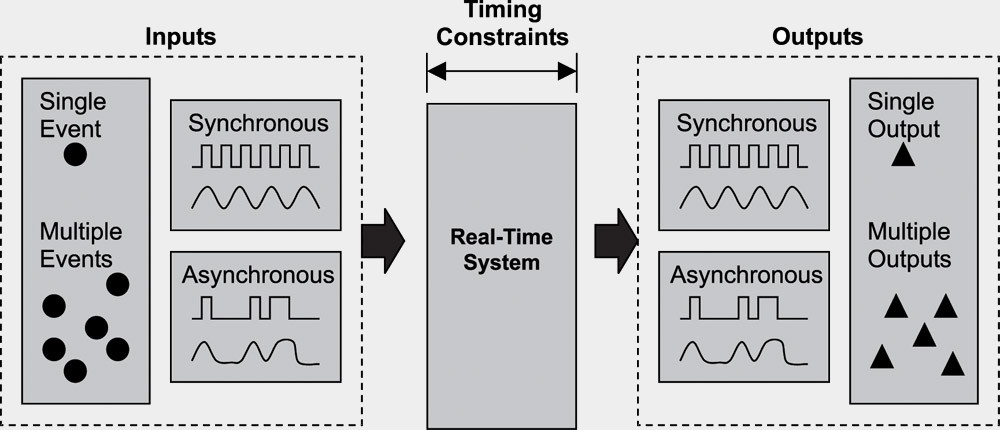
\includegraphics[width=70mm]{images/rts.jpg}

    \end{columns}
\bigskip
\begin{itemize}
\item \textbf{Soft Real Time}: cuando se acepta que los requerimientos de tiempo límite para producir el resultado pueden no cumplirse en algunas ocasiones.
\bigskip
\item \textbf{HARD Real Time}: cuando los requerimientos de tiempo límite de respuesta a un evento deben cumplirse siempre.
\bigskip
 \item[Manipulador] (Ejemplo): {\small \url{https://youtu.be/v26tDdINop4?t=46}}
\end{itemize}
\end{frame}







\begin{frame}{Sistema de Tiempo Real (RTS)}

   \begin{columns}[onlytextwidth,T]
     \column{\dimexpr\linewidth-70mm-5mm}

\begin{itemize}
  \item[RTS] cuando la correctitud del sistema depende:

\bigskip
(1) del resultado lógico de la computación, y

\bigskip
(2) del tiempo que toma producir el resultado.

\bigskip
  \item[FALLO] \textit{Si una restricción de tiempo no se cumplió, el sistema falló (aunque se haya cumplido billones de veces anteriormente).}

\end{itemize}

      \column{70mm}
    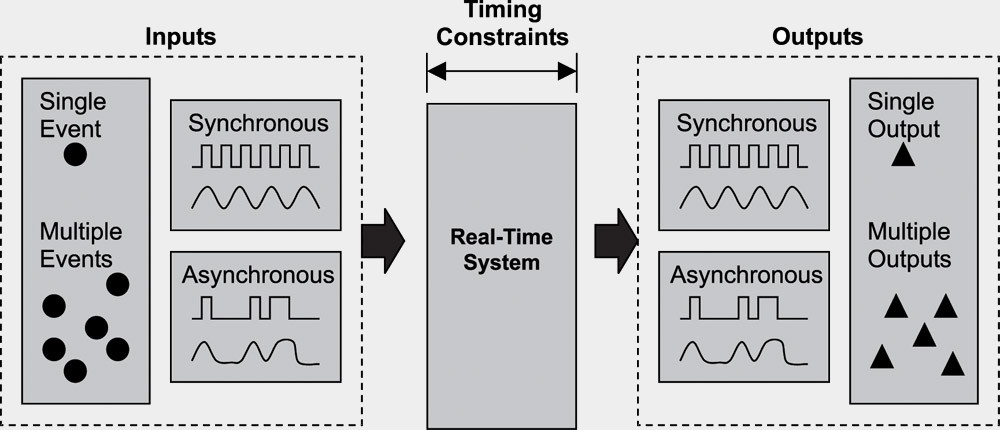
\includegraphics[width=70mm]{images/rts.jpg}

    \end{columns}
\bigskip
    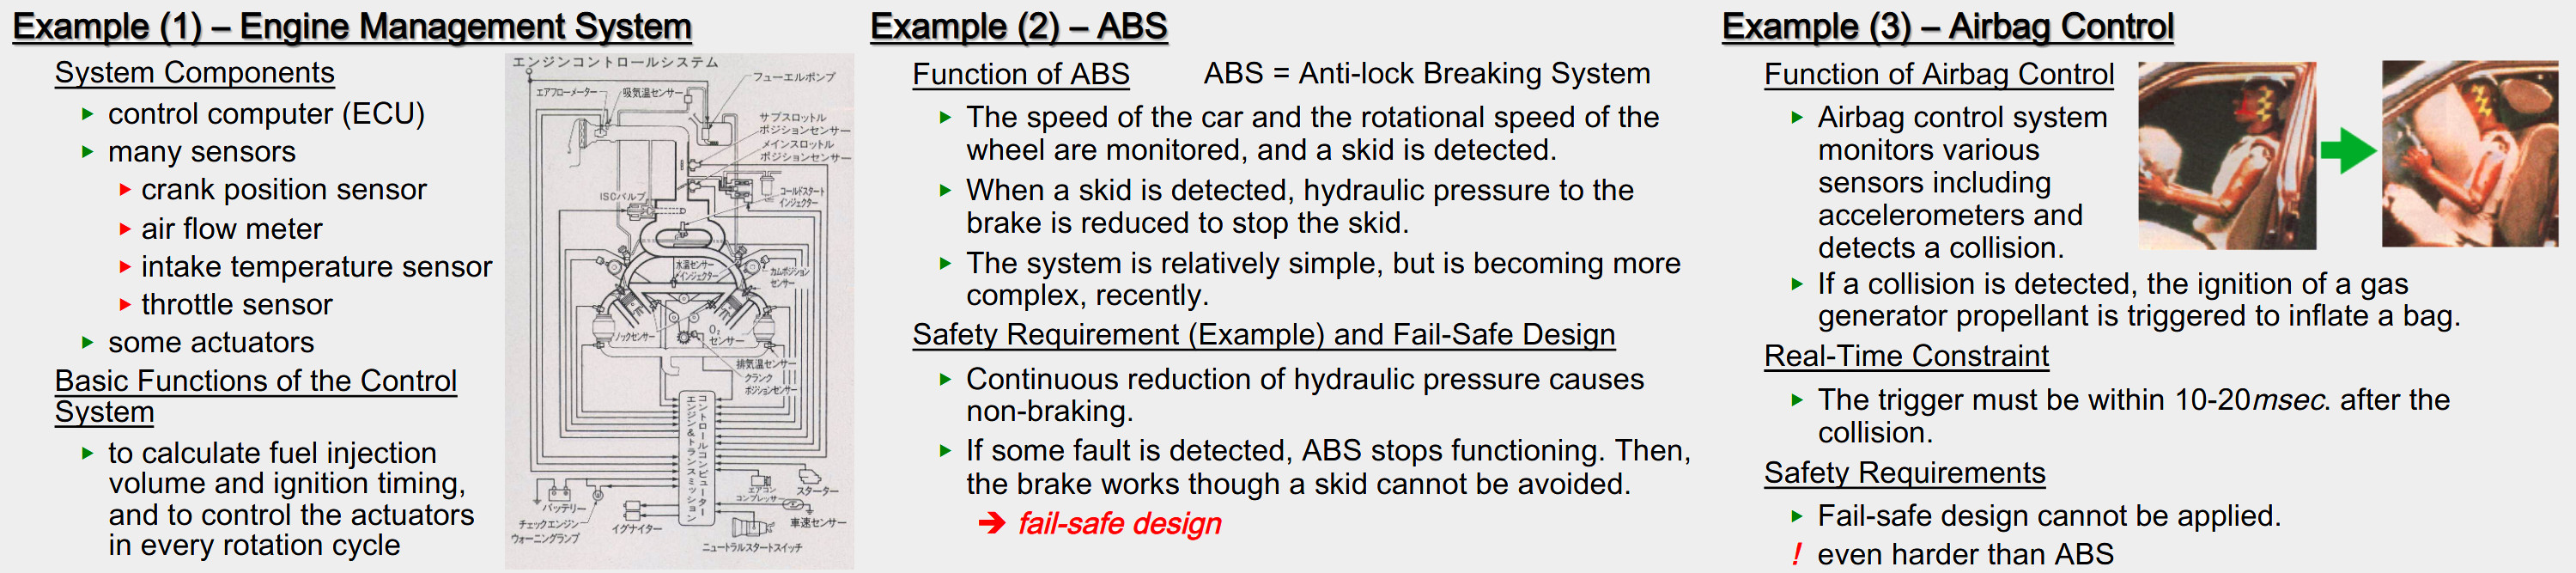
\includegraphics[width=140mm]{images/ejemplos.jpg}

\end{frame}




\begin{frame}{Sistema de Tiempo Real (RTS)}

   \begin{columns}[onlytextwidth,T]
     \column{\dimexpr\linewidth-70mm-5mm}

\begin{itemize}
  \item[RTS] cuando la correctitud del sistema depende:

\bigskip
(1) del resultado lógico de la computación, y

\bigskip
(2) del tiempo que toma producir el resultado.

\bigskip
  \item[FALLO] \textit{Si una restricción de tiempo no se cumplió, el sistema falló (aunque se haya cumplido billones de veces anteriormente).}

\end{itemize}

      \column{70mm}
    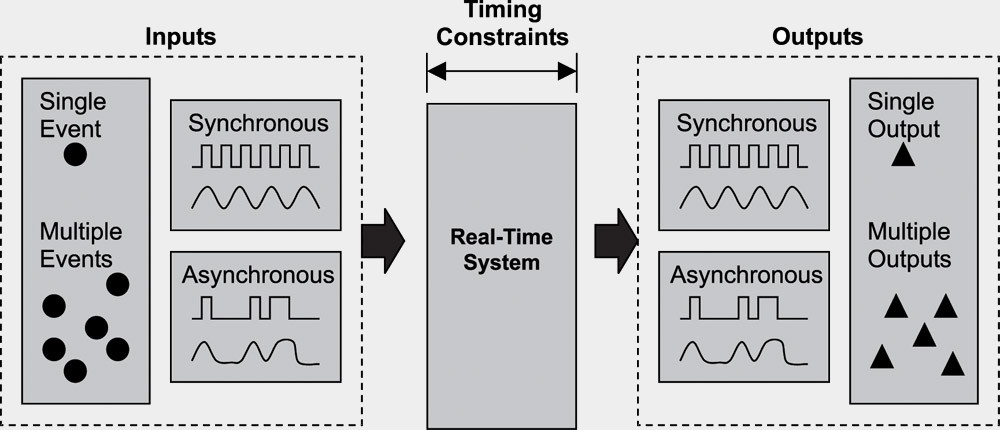
\includegraphics[width=70mm]{images/rts.jpg}

    \end{columns}
\bigskip
    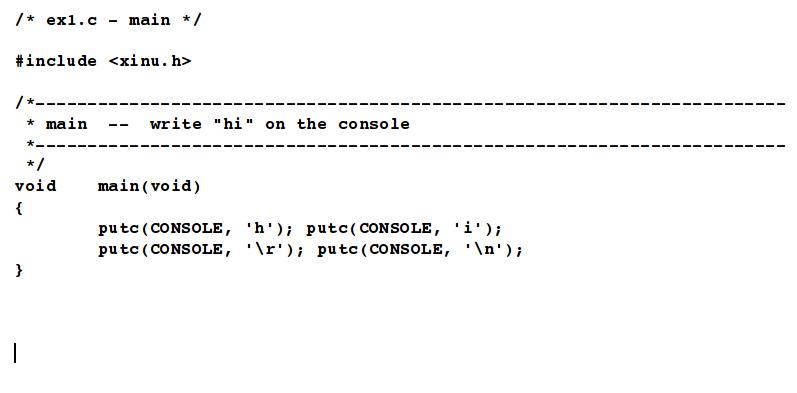
\includegraphics[width=140mm]{images/ejemplo1.jpg}

\end{frame}



\begin{frame}{Sistema de Tiempo Real (RTS)}

   \begin{columns}[onlytextwidth,T]
     \column{\dimexpr\linewidth-70mm-5mm}

\begin{itemize}
  \item[RTS] cuando la correctitud del sistema depende:

\bigskip
(1) del resultado lógico de la computación, y

\bigskip
(2) del tiempo que toma producir el resultado.

\end{itemize}

      \column{70mm}
    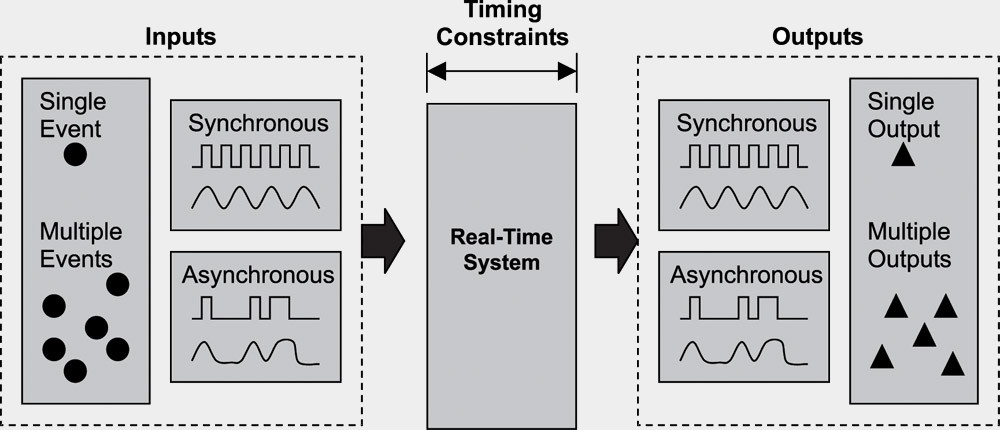
\includegraphics[width=70mm]{images/rts.jpg}

    \end{columns}
\bigskip
El siguiente ejemplo: \textbf{¿Es un sistema de tiempo real?}
\bigskip
    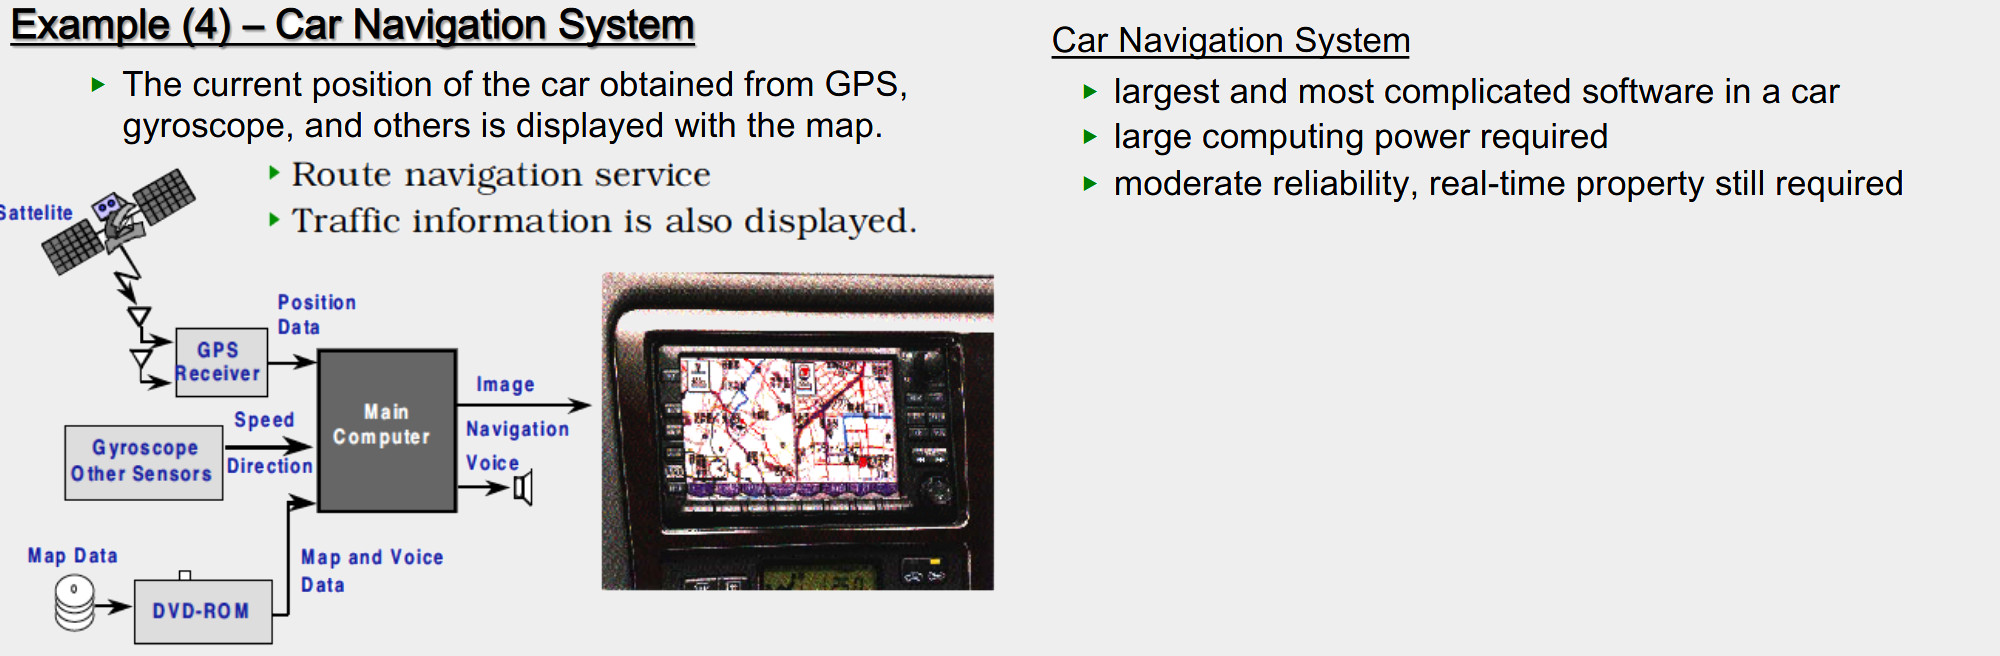
\includegraphics[width=120mm]{images/ejemplo4.jpg}

\end{frame}





\begin{frame}{Sistema Operativo de Tiempo Real}

   \begin{columns}[onlytextwidth,T]
     \column{\dimexpr\linewidth-50mm-5mm}

\begin{itemize}
  \item[RTOS] incluyen las siguientes características:

\bigskip
(1) Cambio de contexto veloz.

\bigskip
(2) Multitarea con comunicación entre procesos (entre tareas).

\bigskip
(3) Capacidad para responder a las interrupciones externas rapidamente.

\bigskip
(4) Tamaño reducido.

\bigskip
(5) Planificador apropiativo (preemptive scheduling).

\bigskip
(6) Otros.

\bigskip
\bigskip
\end{itemize}
      \column{70mm}
    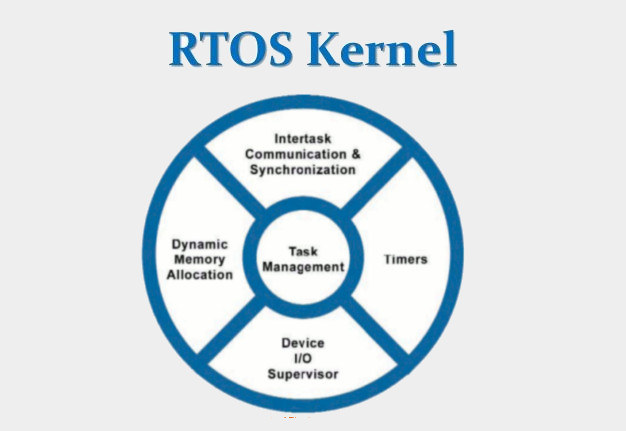
\includegraphics[width=80mm]{images/rtos.jpg}

    \end{columns}
\textit{William Stallings. Operating Systems}

\end{frame}




\begin{frame}{Sistema Operativo de Tiempo Real}

   \begin{columns}[onlytextwidth,T]
     \column{\dimexpr\linewidth-50mm-5mm}

\begin{itemize}
  \item[RTOS] Definido por su planificador (scheduler). \\ El kernel de un RTOS tiene 3 funciones:

\bigskip
(1) El kernel se encarga de las rutinas de atención de interrupciones.

\bigskip
(2) El kernel provee un planificador que determina la secuencia en que las tareas son ejecutadas.

\bigskip
(3) El kernel provee mecanismos de comunicación entre procesos (entre tareas).

\bigskip
\bigskip
\end{itemize}
      \column{70mm}
    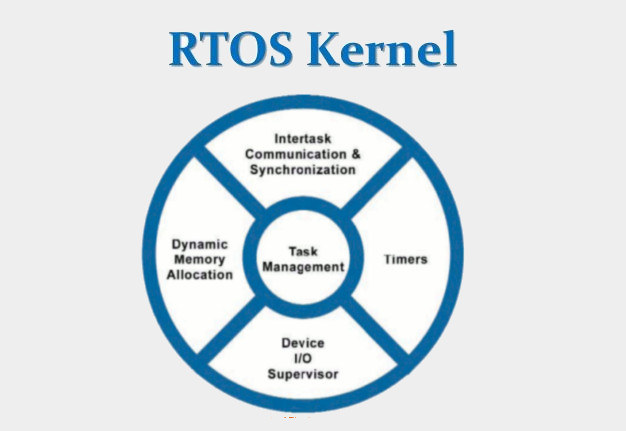
\includegraphics[width=80mm]{images/rtos.jpg}

    \end{columns}
\textit{Alan Clements. Microprocessor System Design: 68000 hardware, software and interfacing}

\end{frame}



\begin{frame}{Sistema Operativo de Tiempo Real}

   \begin{columns}[onlytextwidth,T]
     \column{\dimexpr\linewidth-50mm-5mm}

\begin{itemize}
  \item[RTOS] tiene que soportar algún modo de compartir recursos y los requerimientos de tiempo de las tareas. 

\item Sus funciones son:

\bigskip
(1) Planificador de tareas.

\bigskip
(2) Manejo de interrupciones.

\bigskip
(3) Administración de memoria.

\bigskip
(4) Compartir código entre tareas.

\bigskip
(5) Compartir dispositivos entre tareas.

\bigskip
(6) Sincronización y Comunicación entre procesos.

\bigskip
\bigskip
\end{itemize}
      \column{70mm}
    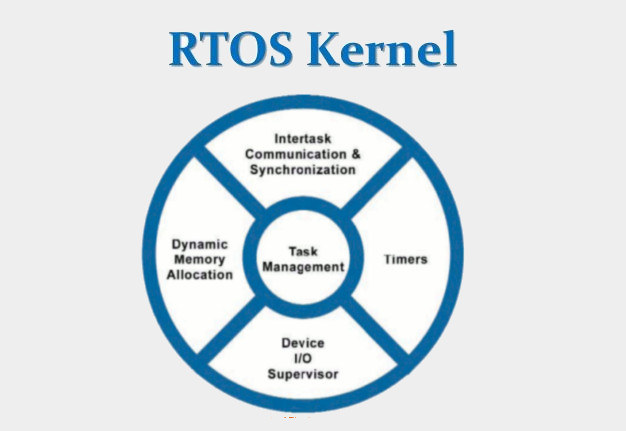
\includegraphics[width=80mm]{images/rtos.jpg}

    \end{columns}

\textit{Stuart Bennet. Real-Time Computer Control: An Introduction}
\end{frame}












\begin{frame}{Sistema Operativo de Tiempo Real}

   \begin{columns}[onlytextwidth,T]
     \column{\dimexpr\linewidth-50mm-5mm}

\begin{itemize}
  \item[RTOS] \textit{Un RTOS es un conjunto de herramientas que posibilita la confección de un sistema: posiblemente embebido, posiblemente de tiempo real, multitarea, posiblemente predecible, y posiblemente determinista. (by pse2020)}

\item Un RTOS provee:

\begin{enumerate}
\item Planificador de tareas apropiativo.

\item Administración de memoria.

\item Administración de la E/S.

\item Comunicación entre procesos y datos compartidos.
\end{enumerate}

\item Un RTOS debe:

\begin{enumerate}
\item Ser predecible.

\item Determinista.
\end{enumerate}


\item Un RTOS suele:

\begin{enumerate}
\item Estar preparado para microcontroladores (o microprocesadores).

\item Venir en modo código fuente.

\item La aplicación embebida de tiempo real se desarrolla mezclada con el código fuente RTOS.

\item Ser predecible asignado prioridades fijas en tiempo de compilación.
\end{enumerate}



\bigskip
\end{itemize}
      \column{70mm}
    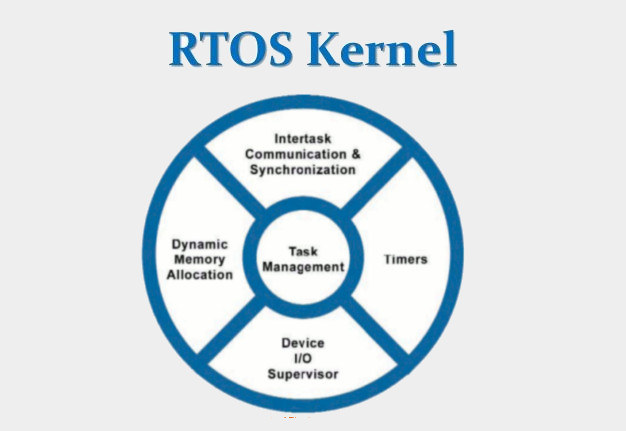
\includegraphics[width=80mm]{images/rtos.jpg}

    \end{columns}

\end{frame}





\begin{frame}{Sistema Operativo de Tiempo Real}

   \begin{columns}[onlytextwidth,T]
     \column{\dimexpr\linewidth-30mm-5mm}

\textbf{Dos definiciones extras (Richar Barry y olvidado):}

\begin{enumerate}

\item  A Real Time Operating System is an operating system that is optimised for use in embedded/real time applications. Their primary objective is to ensure a timely and deterministic response to events. An event can be external, like a limit switch being hit, or internal like a character being received. 
\bigskip

Using a real time operating system allows a software application to be written as a set of independent tasks. Each task is assigned a priority and it is the responsibility of the Real Time Operating System to ensure that the task with the highest priority that is able to run is the task that is running. 

\bigskip
\item An RTOS is an operating system whose internal processes are guaranteed to be compliant with (hard or soft) realtime requirements. The fundamental qualities of a n RTOS are: Predictabe, and Deterministic.

\end{enumerate}

      \column{40mm}
    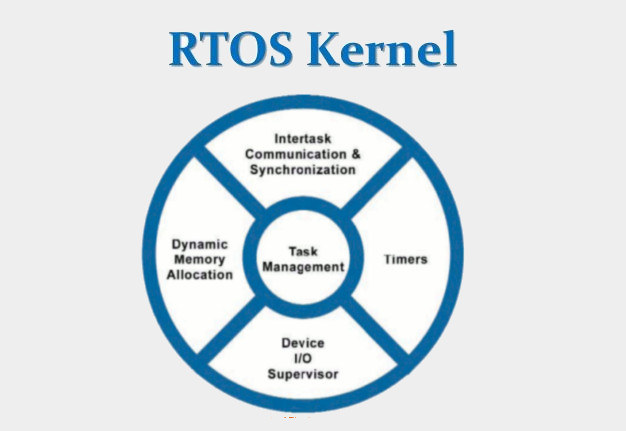
\includegraphics[width=40mm]{images/rtos.jpg}

    \end{columns}

\begin{itemize}
  \item[IMPORTANTE] An RTOS is not a magic wand, your system will not be “realtime” just because you are using an RTOS, what matters is your system design. 
\textcolor{blue}{The RTOS itself is just a toolbox that offers you the required tools for creating a realtime system, you can use the tools correctly or in the wrong way.}
\end{itemize}

\end{frame}


\subsection{¿Por qué utilizar un RTOS?}


\begin{frame}{¿Por qué utilizar un RTOS?}

    \begin{columns}[onlytextwidth,T]
      \column{\dimexpr\linewidth-60mm-5mm}

\begin{itemize}
\item [Resumen] \textit{Porque un RTOS es una excelente herramienta para el desarrollo de un sistema embebido, posiblemente RT.}

\bigskip
\bigskip
\item [Modelo]

\begin{enumerate}
\item El problema se divide en tareas independientes.
\item Si existen tareas relacionadas, un RTOS provee comunicación y sincronización entre tareas.
\item Las regiones críticas pueden ser resueltas con componentes del RTOS.
\item El sistema puede ser diseñado con tareas actividadas mediante eventos \\ (activadas por el scheduler).
\item Las tareas se planifican de manera predecible \\ en base a prioridades.
\item Reuso de código para diferentes tareas.
\end{enumerate}

\end{itemize}

      \column{70mm}
     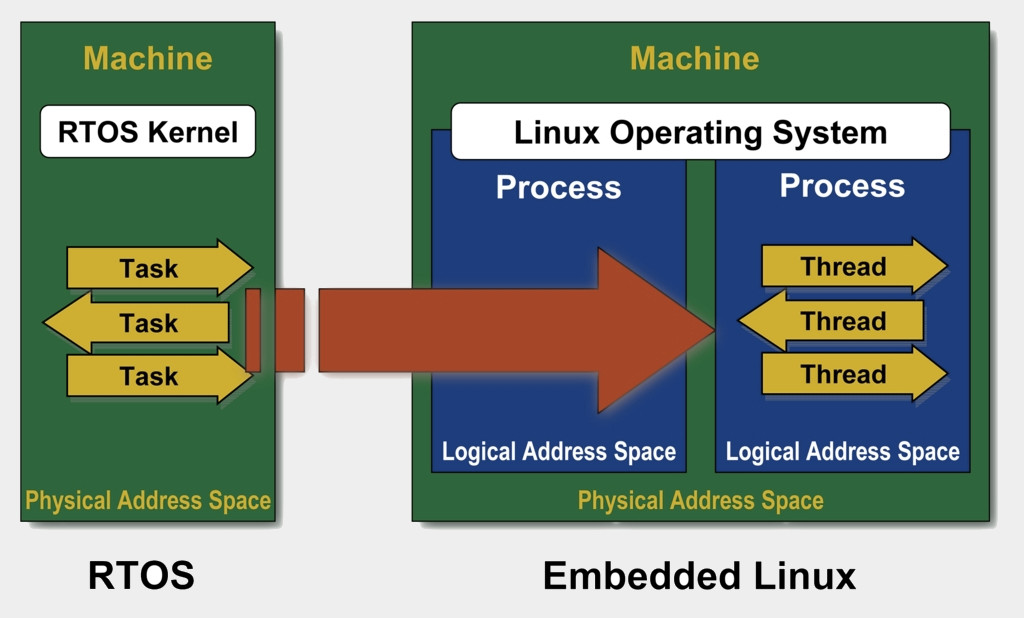
\includegraphics[width=70mm]{images/rtos-vs-linux.jpg}

    \end{columns}
\end{frame}








\subsection{3 maneras de desarrollar un sistema embedido}


\begin{frame}{3 maneras de desarrollar un sistema embebido}

    \begin{columns}[onlytextwidth,T]
      \column{\dimexpr\linewidth-70mm-5mm}

\begin{itemize}
\item [Ejemplo] \textit{Un sistema embebido que controla una planta quimica.}

\bigskip
Presenta una interfaz al usuario con LCD, teclado y leds. 

\bigskip
Tambien una interfaz web para verificar el estado de la planta remotamente.

\end{itemize}

      \column{75mm}

     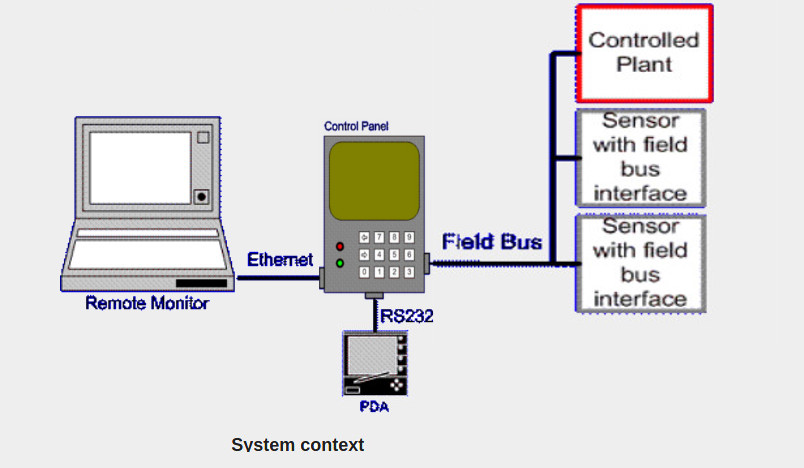
\includegraphics[width=80mm]{images/hipotetico-sistema2.jpg}
    \end{columns}
\end{frame}

\begin{frame}{3 maneras de desarrollar un sistema embebido}

\begin{itemize}
\item [Ejemplo] \textit{Un sistema embebido que controla una planta (o experimento químico). Presenta una interfaz al usuario con LCD, teclado y leds. Tambien una interfaz web para control remoto.}
\end{itemize}

    \begin{columns}[onlytextwidth,T]
      \column{\dimexpr\linewidth-70mm-5mm}


\begin{itemize}
\item [Loop+Timers]

\begin{enumerate}
\item Las tareas de interfaz fisica se realizan en un bucle infinito en main.
\item Dos tareas controladas por software timers: una que lee los sensores y controla la planta; y otra que recibe o envía por la interfaz web.
\end{enumerate}
\end{itemize}


      \column{70mm}

\begin{itemize}
\item [RTOS]

\begin{enumerate}
\item El probema se divide en tareas independientes.
\item Cada tarea se ejecuta sólo si sucede un evento que les interese.
\item Cada tarea tiene una prioridad.
\end{enumerate}

\end{itemize}
    \end{columns}
     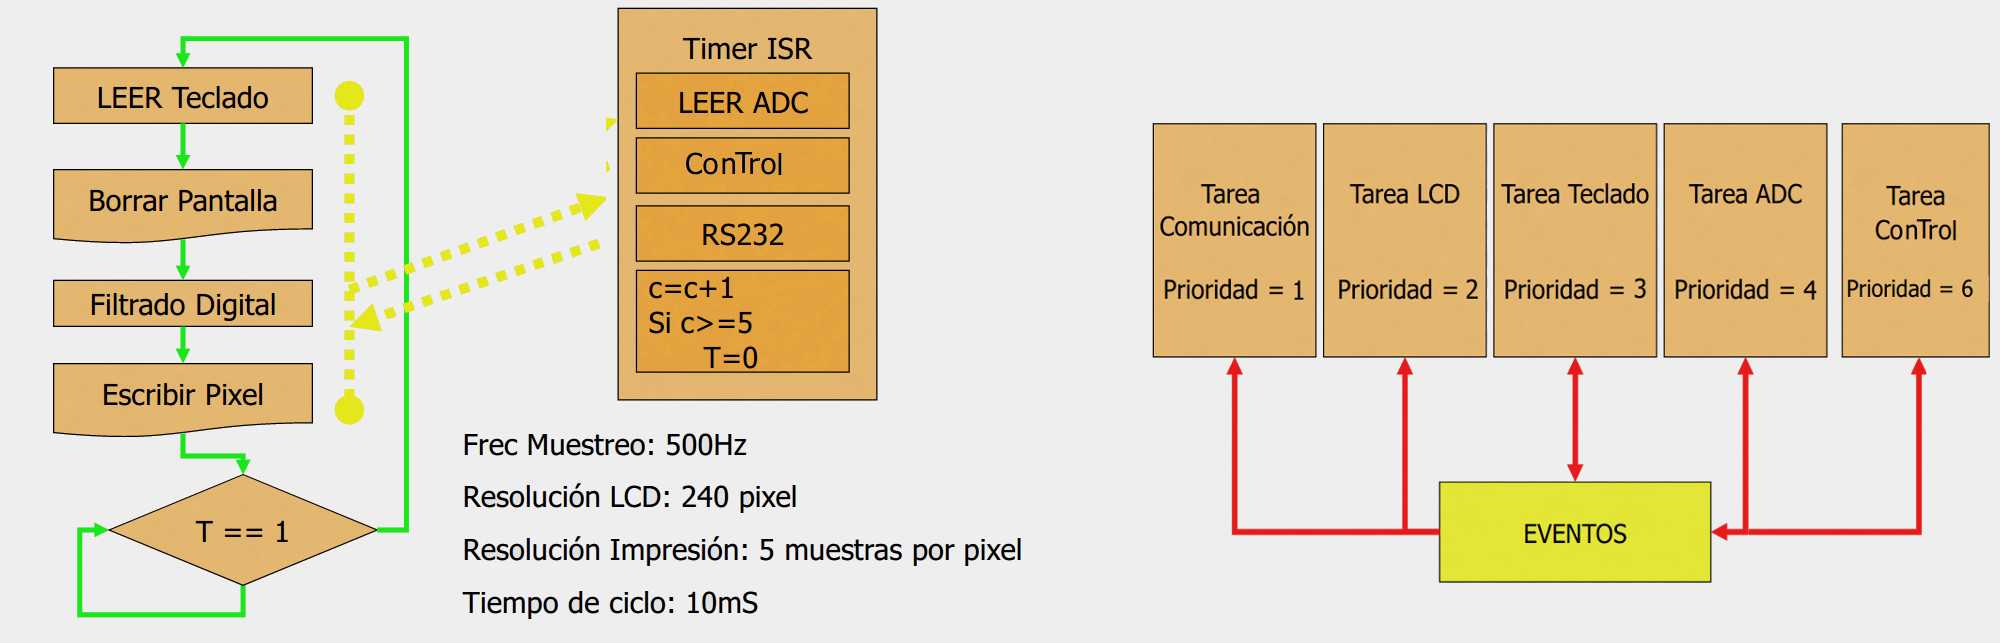
\includegraphics[width=140mm]{images/loop-vs-rtos.jpg}
\end{frame}







\begin{frame}{3 maneras de desarrollar un sistema embebido}{Refinando el modelo con RTOS}


    \begin{columns}[onlytextwidth,T]
      \column{\dimexpr\linewidth-60mm-5mm}

\begin{itemize}
\item [Ejemplo] \textit{Un sistema embebido que controla una planta (o experimento químico). Presenta una interfaz al usuario con LCD, teclado y leds. Tambien una interfaz web para control remoto.}
\end{itemize}

\begin{itemize}

\item [Diseño]

\begin{enumerate}
\item El probema se divide en tareas independientes.
\item Cada tarea se ejecuta sólo si sucede un evento (o más) de interés;
\item o regularmente para, por ejemplo, adquirir señales.
\item Cada tarea tiene una prioridad.
\end{enumerate}


\bigskip

\item [RTOS]
\begin{enumerate}
\item Las tareas Control, LCD y Comunicaciones duermen esperando un evento.
\item Las tareas KEY y ADC adquieren y procesan señales.
\item Las tareas KEY y ADC generan eventos si se debe \textit{actuar}.
\item Las tareas son ejecutadas concurrentemente por el RTOS.
\item Los eventos son semáforos y mailboxes provistos por el RTOS.
\item El planificador del RTOS despierta las tareas dormidas cuando el evento esperado está listo.
\item El planificador RTOS ejecuta las tareas en base a la prioridad.
\item El planificador RTOS permite compartir recursos entre tareas de manera segura.
\end{enumerate}


\end{itemize}

      \column{60mm}

     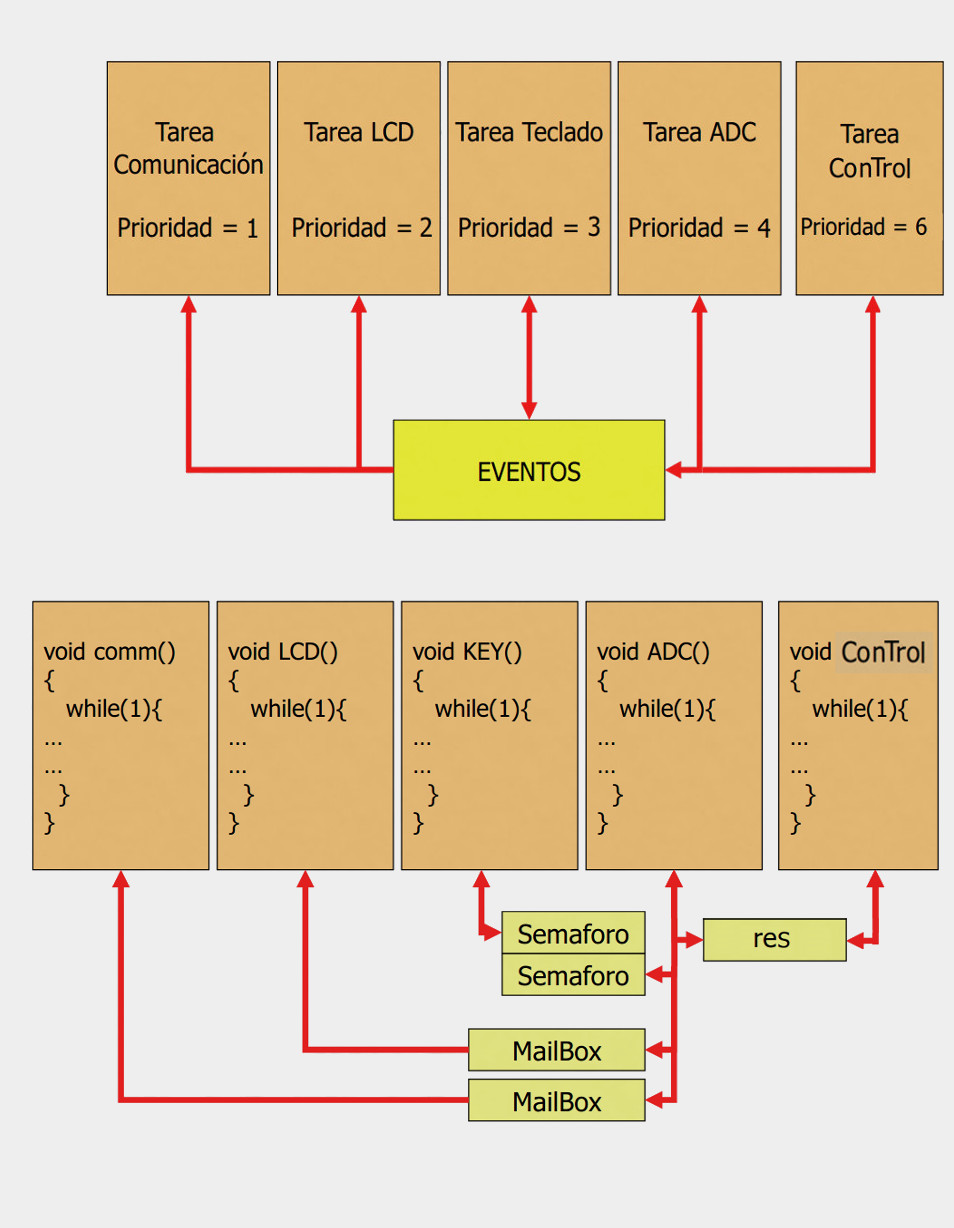
\includegraphics[width=60mm]{images/ejemplo-tareas2.jpg}
    \end{columns}
\end{frame}




\subsection{Introducción a Xinu (características)}
\subsubsection{Servicios que proporciona al desarrollador (sleep)}







\begin{frame}{Xinu}

    \begin{columns}[onlytextwidth,T]
      \column{\dimexpr\linewidth-70mm-5mm}

\begin{small}
	\begin{itemize}
\item[Xinu] Es un \textbf{sistema operativo} pequeño y elegante \\ (fácil de comprender), desarrollado originalmente por Douglas Comer en la Universidad de Purdue, a fines de los 70. 
\item[Versiones] Actualmente existen versiones para \textit{x86 (PC), ARM, MIPS, AVR, y maquinas virtuales}. 
\item[USO] \textit{Académico, en investigación y en la industria}.

\bigskip
Como el tamaño del código fuente es pequeño \\ \textcolor{blue}{Xinu es adecuado en sistemas embebidos.}
\bigskip
\item [web] Mas información:
\begin{enumerate}
\item \textcolor{blue}{\footnotesize \url{https://xinu.cs.purdue.edu/}}
\item \textcolor{blue}{\footnotesize \url{http://se.fi.uncoma.edu.ar/xinu-avr/}}
\item \textit{Douglas Comer, Operating System Design - The Xinu Approach, Second Edition CRC Press, 2015. ISBN 9781498712439}
\end{enumerate}
	\end{itemize}

\end{small}


      \column{70mm}
     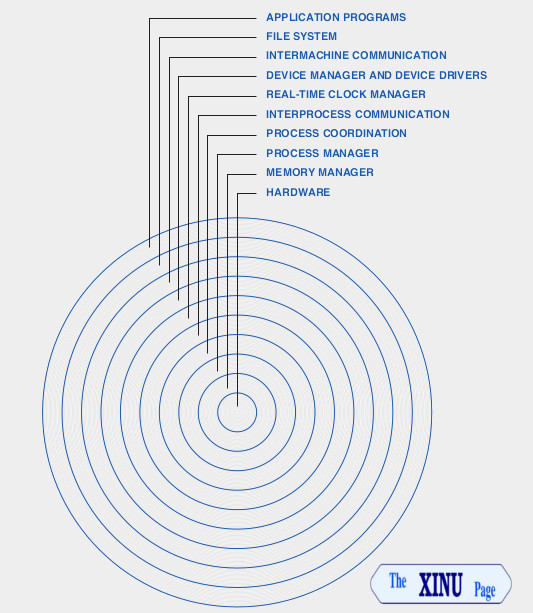
\includegraphics[width=60mm]{images/xinu.jpg}

    \end{columns}
\end{frame}


\begin{frame}{Douglas Comer}

    \begin{columns}[onlytextwidth,T]
      \column{\dimexpr\linewidth-70mm-5mm}

\begin{small}
	\begin{itemize}
\item Ha escrito una decena de libros sobre Sistemas Operativos, Arquitectura de Computadoras y Redes. 

\item Considerado el padre académico de internet:

\begin{itemize}
\item Sus 3 vólumenes sobre redes TCPI/IP en los 80 son considerados la autoridad de referencia de los protocolos de Internet.

\bigskip
\item Jugaron un rol clave en popularizar esos protocolos, haciéndolos entendibles a la generación de ingenieros y técnicos que se formaron previo a internet.
\end{itemize}

\bigskip
\begin{itemize}
\item \textcolor{blue}{\footnotesize \url{https://www.cs.purdue.edu/homes/comer/}}
\item \textcolor{blue}{comer@purdue.edu}
\end{itemize}
\end{itemize}

\end{small}


      \column{70mm}
     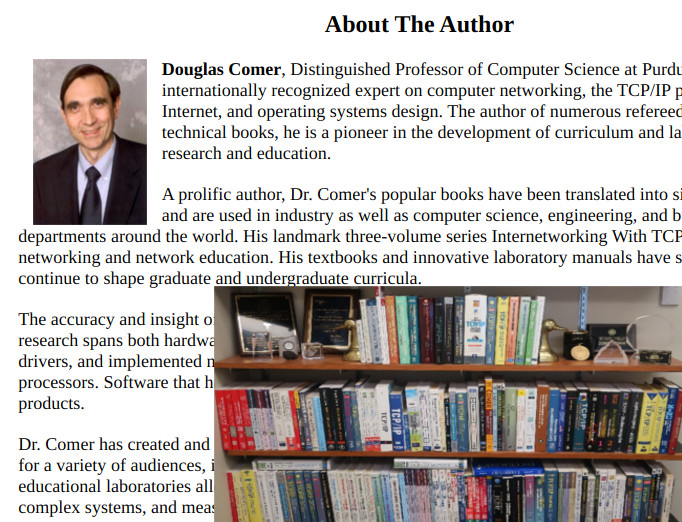
\includegraphics[width=60mm]{images/douglas.jpg}

    \end{columns}
\end{frame}





\begin{frame}{Xinu}

    \begin{columns}[onlytextwidth,T]
      \column{\dimexpr\linewidth-70mm-5mm}

\begin{small}
	\begin{itemize}
\item[Xinu] Es un \textbf{sistema operativo} pequeño y elegante \\ (fácil de comprender), desarrollado originalmente por Douglas Comer en la Universidad de Purdue, a fines de los 70. 
\bigskip
  \item[Características] Xinu provee:
\begin{enumerate}
\item Creación dinámica de procesos (threads).
\item Asignación dinámica de memoria.
\item Administración del real-time clock.
\item Coordinación y sincronización de procesos.
\item Un planificador apropiativo multi-tarea (preemptive multi-tasking).
\item Sistemas de archivos locales y remotos.
\item Un shell (si es necesario).
\item Funciones de E/S (API) independientes del dispositivo.
\item Una pila de protocolos TCP/IP.
\end{enumerate}
	\end{itemize}

\end{small}


      \column{70mm}
     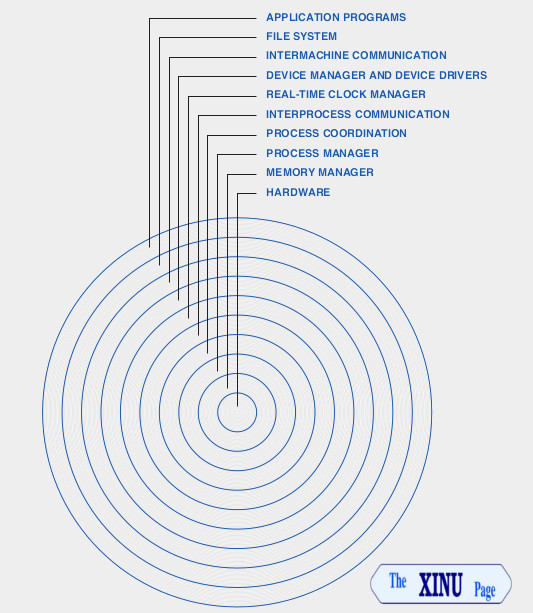
\includegraphics[width=60mm]{images/xinu.jpg}

    \end{columns}
\end{frame}














\begin{frame}{Xinu}

    \begin{columns}[onlytextwidth,T]
      \column{\dimexpr\linewidth-50mm-5mm}

\begin{small}
	\begin{itemize}
\item [OS style]Los sistemas operativos multitarea pueden ser:
\begin{itemize}
\item de Tiempo Compartido
\item de Tiempo-Real
\end{itemize}

\item [Xinu RTOS] Xinu utiliza fixed-priority, y coloca en ejecución al proceso de mas alta prioridad, lo que lo categoriza como RTOS.

\bigskip
\item [Planificador] Su planificador (scheduler) puede ser apropiativo (preemptive) o cooperativo.

\bigskip
\item [Concurrente] El desarrollo de la aplicación se debe realizar teniendo en cuenta detalles de la programación concurrente.

	\end{itemize}

     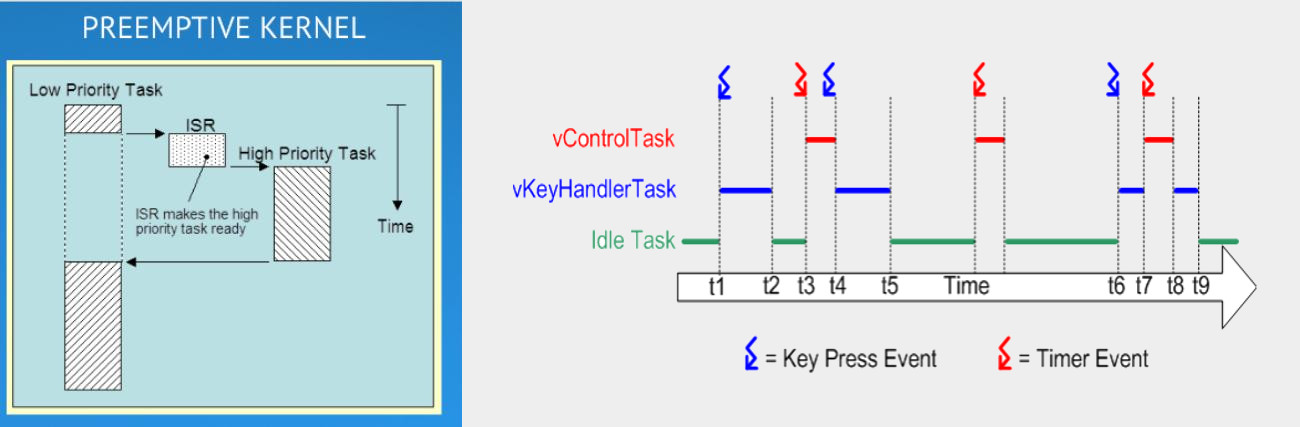
\includegraphics[width=100mm]{images/preemptive.jpg}
\end{small}


      \column{50mm}
     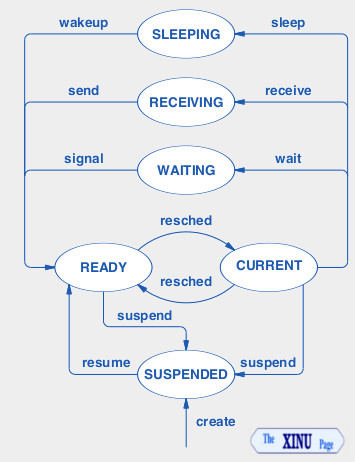
\includegraphics[width=40mm]{images/estados.jpg}

    \end{columns}
\end{frame}


\subsection{Gestión de Tareas en Xinu (planificador/scheduler RTOS)}

\begin{frame}{Tareas en Xinu}


    \begin{columns}[onlytextwidth,T]
      \column{\dimexpr\linewidth-60mm-5mm}


	\begin{itemize}
\item [modelo] \textbf{Xinu sigue el modelo de threads.}
\item [tareas] 
\begin{itemize}
\item Cada tarea (proceso o thread) tiene su propia pila y contexto, pero comparte el segmento de código y segmento de datos.
\bigskip
\item Una tarea es una función en C. Se crea con la llamada al sistema \textbf{create()}, el cual recibe como argumento el nombre de la función.
\bigskip 
\item Se pueden crear muchas tareas a partir de una misma función (posiblemente con diferentes argumentos).
\end{itemize}

\item[API]

\begin{itemize}
\bigskip
\item \textbf{create(args)} y \textbf{resume(pid)} crean una tarea y la colocan en estado de \textit{LISTO}.

\bigskip
\item \textbf{sleep(n)} y \textbf{sleepms(n)} colocan la tarea en estado \textit{DURMIENDO}.

\bigskip
\item \textbf{kill(d)} permite matar un proceso. Por lo que un proceso puede finalizar con \textbf{kill(}getpid()\textbf{)}.

\bigskip
\item \textbf{suspend(pid)} suspende un proceso.
\end{itemize}
\end{itemize}

      \column{50mm}
     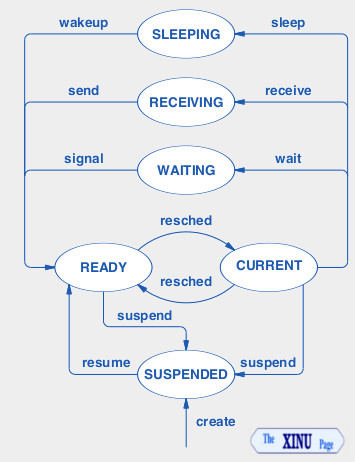
\includegraphics[width=50mm]{images/estados.jpg}

    \end{columns}
\end{frame}





\begin{frame}[fragile]{Xinu: administrador de memoria}

    \begin{columns}[onlytextwidth,T]
      \column{\dimexpr\linewidth-60mm-5mm}

	\begin{itemize}
\bigskip
  \item[Gestor de memoria] En Xinu existe una API para requerir memoria en tiempo de ejecución.

\bigskip
\begin{itemize}
\item Utilizado principalmente por create y kill, para asignar pila a un nuevo proceso (thread).

\bigskip
\item Se puede solicitar un bloque de memoria en ejecución, pero no es recomendado en embebidos y RT.
\end{itemize}

\bigskip
\item[API]

\begin{lstlisting}[language=c,basicstyle=\footnotesize]

getstk(n); 
freestk(b,s);

getmem(n);
freemem(b,s);
\end{lstlisting}

	\end{itemize}

      \column{50mm}
    % \includegraphics[width=50mm]{images/cmos2.png}

    \end{columns}
\end{frame}


\begin{frame}[fragile]{Xinu: dispositivo de E/S console}

    \begin{columns}[onlytextwidth,T]
      \column{\dimexpr\linewidth-60mm-5mm}

	\begin{itemize}
  \item[CONSOLE] La consola en xinu-avr es la terminal del usuario, y está controlada por el driver uart.

\bigskip
\begin{itemize}
\item Xinu ofrece algunas funciones similares al estandar de C, que utilizan la consola (serial/uart en avr) de manera predeterminada.
\item Internamente Xinu utiliza una capa de software de E/S independiente del dispositvo (con funciones open, read, write, seek, putc, close, etc).

\end{itemize}

\bigskip
\item[API] de algunas funciones de biblioteca de Xinu

\begin{lstlisting}[language=c,basicstyle=\footnotesize]

/* son equivalentes */
putchar(ch)     
putc(CONSOLE,(ch))

/* son equivalentes */
getchar(ch)     
getc(CONSOLE,(ch))

printf(args); 

/* todas la anteriores emiten la salida a través del serial uart en avr */
\end{lstlisting}

	\end{itemize}

      \column{50mm}
    % \includegraphics[width=50mm]{images/cmos2.png}

    \end{columns}
\end{frame}


\subsection{Xinu en ejemplos: Tareas}

\subsubsection{Tareas concurrentes}
\subsubsection{Reuso de código}
\subsubsection{Diseño de tiempo real: prioridades fijas}













\begin{frame}[fragile]{Xinu: crear y ejecutar 3 procesos concurrentes}{Programación concurrente}

    \begin{columns}[onlytextwidth,T]
      \column{\dimexpr\linewidth-70mm-5mm}

\begin{small}
	\begin{itemize}
\bigskip
  \item[Secuencia]
\begin{enumerate}
\item Al iniciar Xinu existen 2 procesos en ejecución: main() y null().
\bigskip
\item Cada proceso tiene su propia pila y contexto.
\bigskip
\item main() entonces crea 3 nuevos procesos y finaliza.
\bigskip
\item send\_a(), led() y led\_placa() son procesos \\ con loop infinitos.
\bigskip
\item Los 4 procesos se ejecutan indefinidamente \\ de manera concurrente.
\bigskip
\item \textcolor{blue}{\href{https://youtu.be/Xg1l9pvxluE/}{Video demostrativo}}
\end{enumerate}
	\end{itemize}

\end{small}

      \column{60mm}
     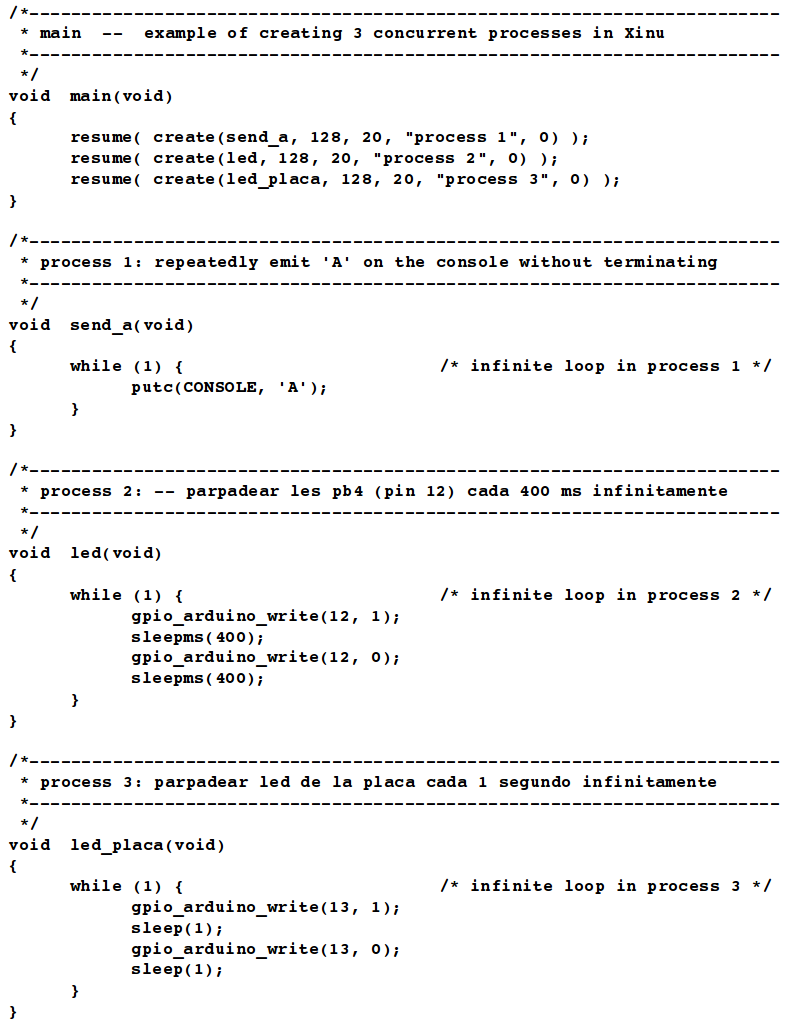
\includegraphics[width=58mm]{images/3tasks.png}

    \end{columns}
\end{frame}







\begin{frame}[fragile]{Xinu: ejemplo 0 \\ Crear y ejecutar una tarea}

    \begin{columns}[onlytextwidth,T]
      \column{\dimexpr\linewidth-70mm-5mm}

\begin{small}
	\begin{itemize}
\bigskip
  \item[Descripción]
\begin{enumerate}
\item \textbf{create()} crea el proceso \textit{ex\_0}
\begin{itemize}
\item El código fuente de este proceso esta implementado en \textbf{example0()}.
\item Recibe 3 argumentos: nargs (la cantidad de argumentos), y 2 argumentos en args.
\end{itemize}

\bigskip
\item Para compilar esta aplicación junto con Xinu: 

\begin{lstlisting}[language=c,basicstyle=\footnotesize]
cd xinu-avr/
cd compile/
make clean
make
make flash
\end{lstlisting}
\bigskip
\item Los printf están configurados para utilizar el dispositivo CONSOLE en Xinu. 

\bigskip
\item En xinu-avr, el dispositivo CONSOLE es el USART.

\bigskip
\item Para observar el output: \textit{cutecom}
\end{enumerate}
	\end{itemize}

\end{small}

      \column{60mm}
     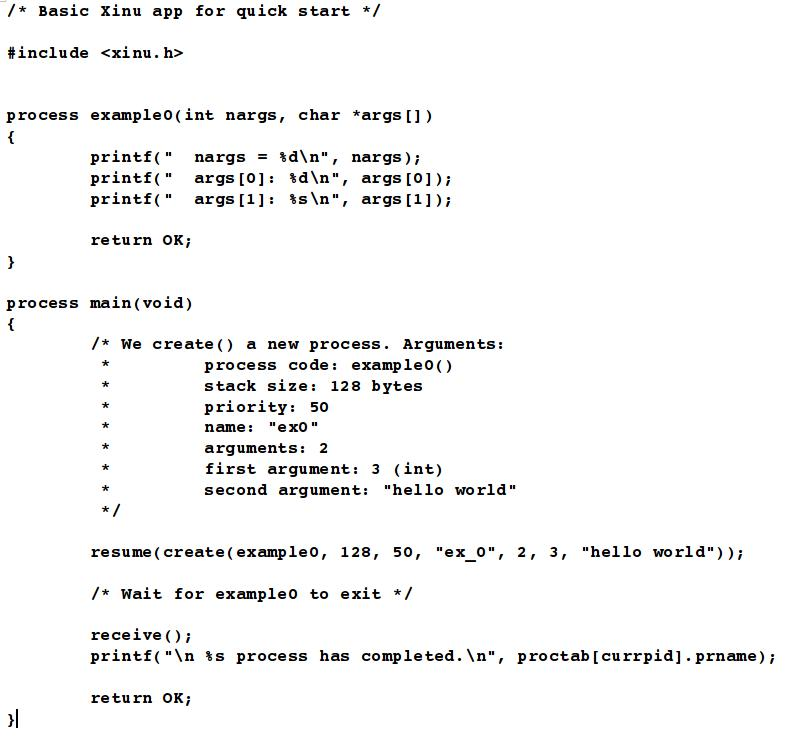
\includegraphics[width=62mm]{images/ejemplo0.jpg}

    \end{columns}
\end{frame}






\begin{frame}[fragile]{Xinu: ejemplo 1 \\ Utilizar putc con el dispositivo CONSOLE}

    \begin{columns}[onlytextwidth,T]
      \column{\dimexpr\linewidth-70mm-5mm}

\begin{small}
	\begin{itemize}
\bigskip
  \item[Descripción]
\begin{enumerate}
\item \textbf{main()} hace uso de la función de biblioteca \textbf{putc()}

\bigskip
\item Para compilar esta aplicación junto con Xinu: 

\begin{lstlisting}[language=c,basicstyle=\footnotesize]
cd xinu-avr/
cd compile/
make clean
make
make flash
\end{lstlisting}
\bigskip
\item Las funciones vistas hasta el momento:

\begin{lstlisting}[language=c,basicstyle=\footnotesize]
create() : system call para crear un proceso y dejarlo en estado SUSPENDIDO
resume(): función de Xinu para colocar el proceso en estado de LISTO
nargs y args[]: argumentos de entrada de un proceso
putc(): función de biblioteca para enviar un char a un dispositivo
printf(): función de biblioteca para enviar un output a CONSOLE
\end{lstlisting}

\bigskip
\item En xinu-avr, el dispositivo CONSOLE es el USART.

\bigskip
\item Para observar el output: \textit{cutecom}
\end{enumerate}
	\end{itemize}

\end{small}

      \column{60mm}
     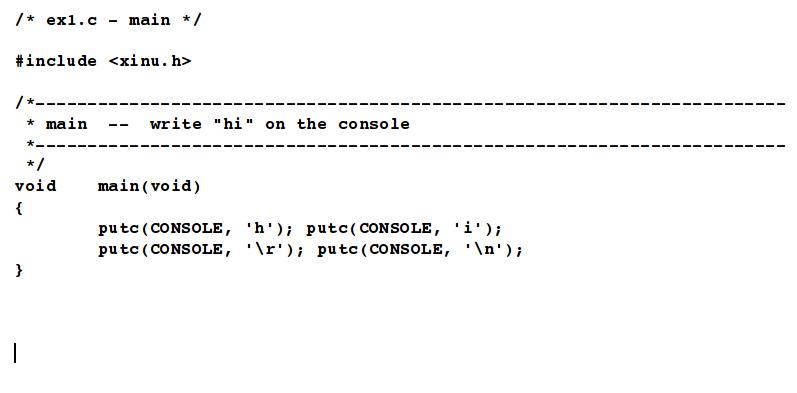
\includegraphics[width=62mm]{images/xinu-ejemplo1.jpg}

    \end{columns}
\end{frame}









\begin{frame}[fragile]{Xinu: ejemplo 2 \\ Tareas concurrentes}

    \begin{columns}[onlytextwidth,T]
      \column{\dimexpr\linewidth-70mm-5mm}

\begin{small}
	\begin{itemize}
\bigskip
  \item[Descripción]
\begin{enumerate}
\item \textbf{main()} crea dos procesos: sndA y sndB.
	\begin{itemize}
\item Cada proceso tiene un bucle infinito.
\item Cada proceso envía de manera independiente una letra indefinidamente.
	\end{itemize}

\bigskip
\item Para observar el output: \textit{cutecom}
\bigskip
\item Observación: el codigo fuente de un proceso es de tipo void o process.
\end{enumerate}
	\end{itemize}

\end{small}

      \column{70mm}
     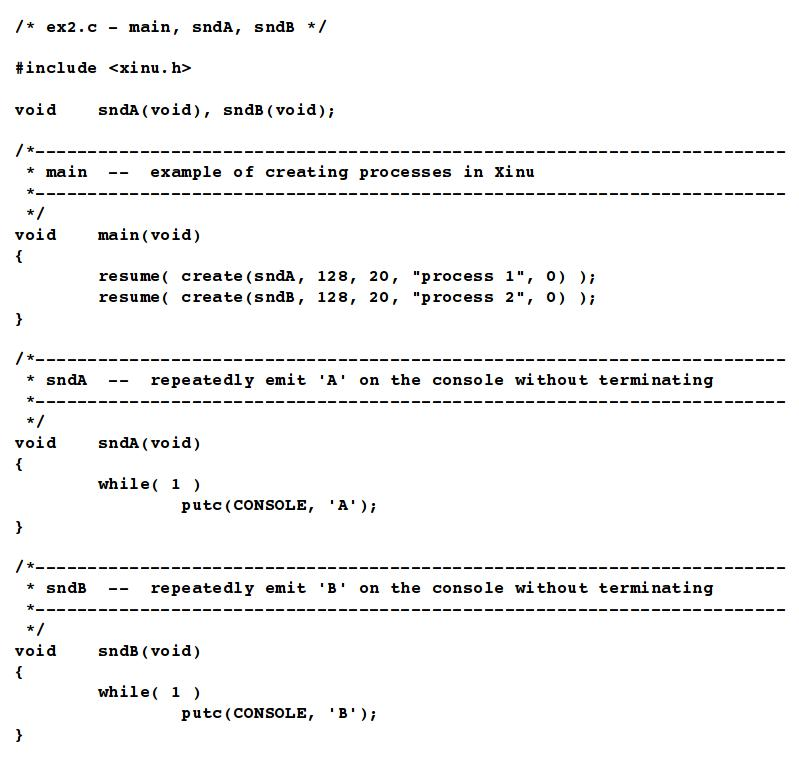
\includegraphics[width=70mm]{images/ejemplo2.jpg}

    \end{columns}
\end{frame}











\begin{frame}[fragile]{Xinu: ejemplo 3 \\ Reuso de código}

    \begin{columns}[onlytextwidth,T]
      \column{\dimexpr\linewidth-70mm-5mm}

\begin{small}
\begin{itemize}
\bigskip
  \item[Descripción]
\begin{enumerate}
\item \textbf{main()} crea y ejecuta dos procesos independientes que utilizan el mismo código (pero con diferentes argumentos).
	\begin{itemize}
\item Cada proceso recibe un argumento (letra A o B).
\item Cada proceso envía de manera independiente su letra indefinidamente.
	\end{itemize}

\bigskip
\item Para observar el output: \textit{cutecom}
\bigskip
\item Observación: el codigo fuente de un proceso es de tipo void o process.
\end{enumerate}
	\end{itemize}

\end{small}

      \column{70mm}
     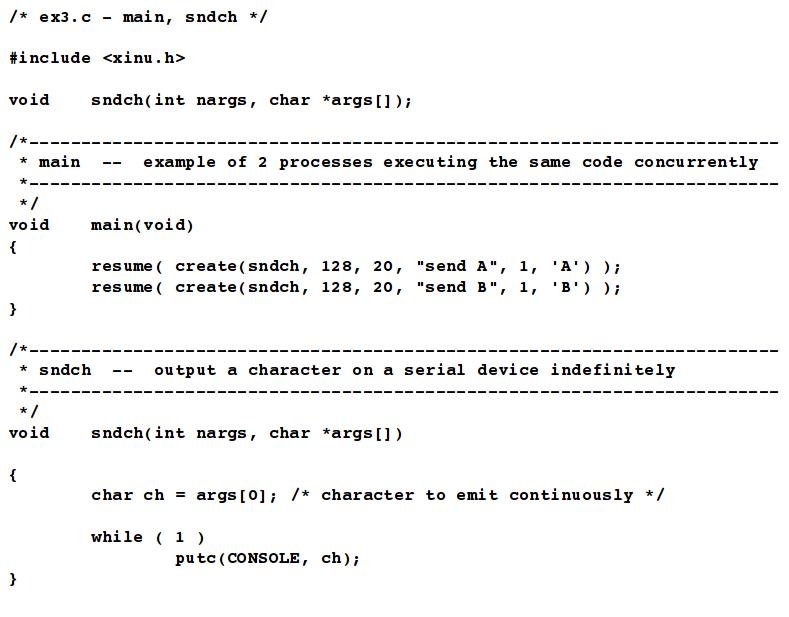
\includegraphics[width=70mm]{images/ejemplo3.jpg}

    \end{columns}
\end{frame}





\subsection{Xinu en ejemplos: Sincronización y Comunicación de Tareas en Xinu}
\subsubsection{Sincronización: semáforos (ej. productor/consumidor)}
\subsubsection{Región crítica: solución con mutex}
\subsubsection{Comunicación: pasaje de mensajes con mailbox}
\subsubsection{Buffers y colas: ports}










\begin{frame}[fragile]{Xinu: ejemplo 4 \\ Productor/Consumidor NO SINCRONIZADOS!}

    \begin{columns}[onlytextwidth,T]
      \column{\dimexpr\linewidth-70mm-5mm}

\begin{small}
\begin{itemize}
\bigskip
  \item[Descripción]
\begin{enumerate}
\item \textbf{main()} crea dos tareas, un productor y un consumidor.
	\begin{itemize}
\item La tarea productora genera 2000 valores de n.
\item La tarea consumidora muestra por CONSOLA el valor de n producido.
	\end{itemize}

\bigskip
\item El sistema falla en su objetivo.\\ La E/S es miles de veces mas lenta que la CPU.
\bigskip
\item Para observar el output: \textit{cutecom}
\bigskip
\item Observación: el codigo fuente de un proceso es de tipo void o process.
\end{enumerate}
	\end{itemize}

\end{small}

      \column{70mm}
     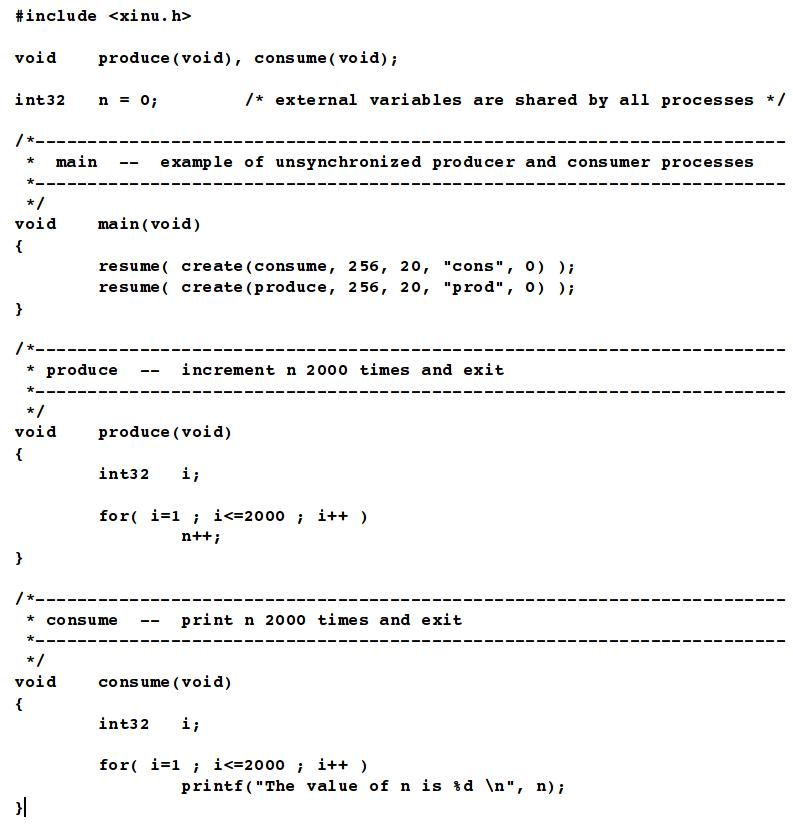
\includegraphics[width=66mm]{images/xinu-ejemplo4.jpg}

    \end{columns}
\end{frame}






\begin{frame}[fragile]{Xinu: ejemplo 4 \\ Sincronización entre tareas (Productor/Consumidor)}

    \begin{columns}[onlytextwidth,T]
      \column{\dimexpr\linewidth-70mm-5mm}

\begin{small}
\begin{itemize}
\bigskip
  \item[Descripción]
\begin{enumerate}
\item \textbf{main()} crea dos tareas, un productor y un consumidor.
	\begin{itemize}
\item La tarea productora genera 2000 valores de n.
\item La tarea consumidora muestra por CONSOLA el valor de n producido.
	\end{itemize}

\bigskip
\item Solución clásica al problema productor/consumidor, utilizando dos semáforos. \\ Las tareas están ahora sincronizadas.

\bigskip
\item \textbf{\textit{\textcolor{blue}{Xinu provee semáforos para sincronización}}}
\bigskip
\item Para observar el output: \textit{cutecom}
\end{enumerate}
	\end{itemize}

\end{small}

      \column{70mm}
     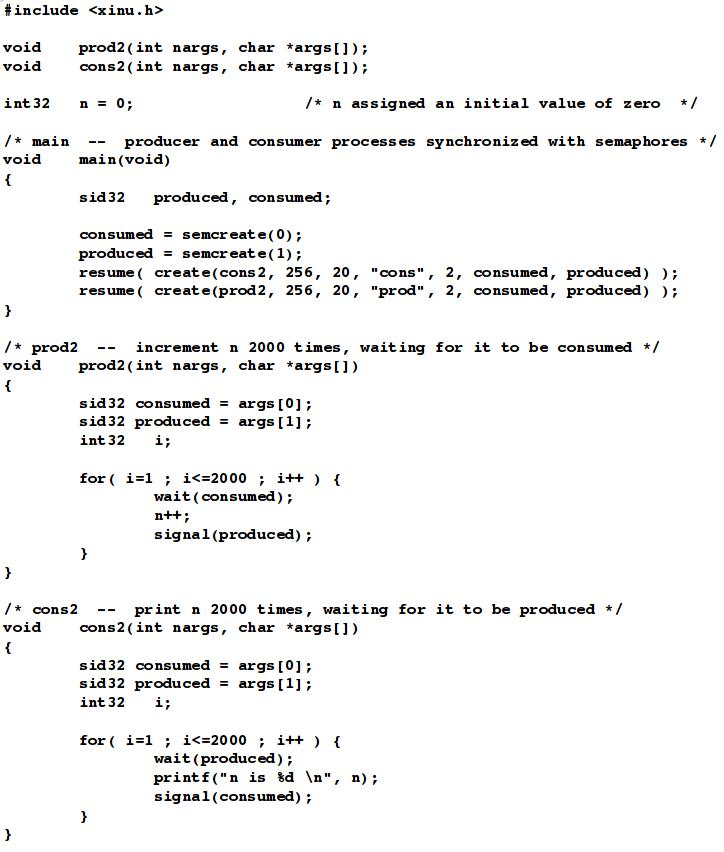
\includegraphics[width=60mm]{images/xinu-ejemplo5.jpg}

    \end{columns}
\end{frame}





\begin{frame}[fragile]{Xinu: Semáforos y mutex. Región crítica. Ejemplo de uso.}

    \begin{columns}[onlytextwidth,T]
      \column{\dimexpr\linewidth-70mm-5mm}

\begin{itemize}
  \item[Descripción]
\begin{enumerate}
\begin{footnotesize}
\item Un buffer circular es una excelente herramienta de comunicación entre dos procesos.
\item Una tarea produce elementos.
\item Una tarea remueve elementos y los procesa. Si no hay elementos en el buffer la tarea consumidora bloquea.
\item Los semáforos se utilizan para controlar los límites del buffer.
\item El mutex se utiliza para proteger la región crítica.
\item \textbf{\textit{\textcolor{blue}{En Xinu, un mutex puede ser implementado utilizando un semáforo binario correctamente utilizado. \\ Se debe prestar especial atención a esta implementación.}}}
\end{footnotesize}
\end{enumerate}
\end{itemize}

     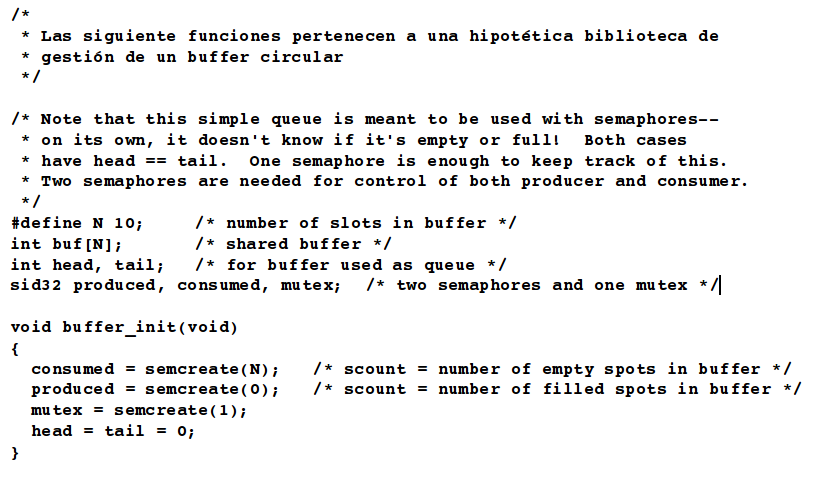
\includegraphics[width=70mm]{images/mutex-sem1.png}

      \column{70mm}
     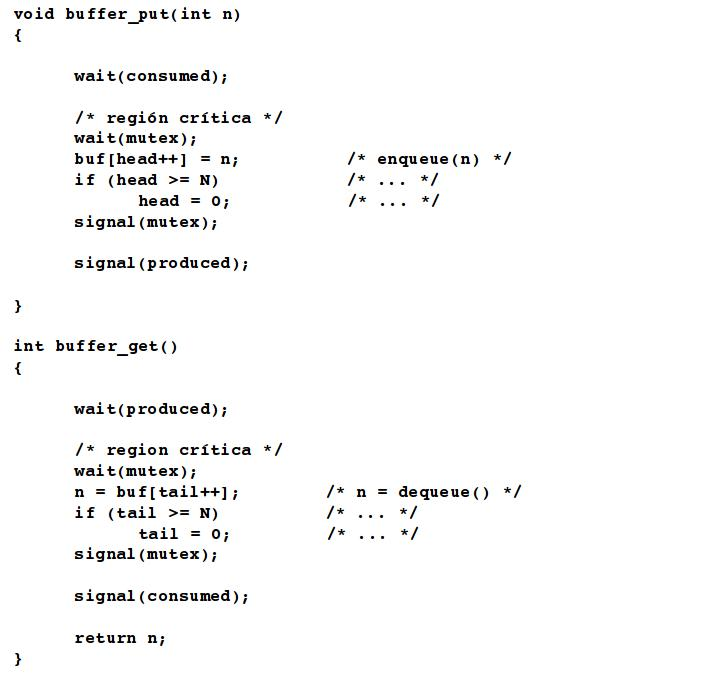
\includegraphics[width=70mm]{images/mutex-sem2.jpg}

    \end{columns}
\end{frame}













\subsection{Recursos}




\begin{frame}{Recursos}

\begin{itemize}

\item [WEB]
\begin{enumerate}
\item \textcolor{blue}{\footnotesize \url{https://xinu.cs.purdue.edu/}}
\item \textcolor{blue}{\footnotesize \url{http://se.fi.uncoma.edu.ar/xinu-avr/}}
\end{enumerate}

\item [LIBRO]

\begin{enumerate}
\item \textit{Douglas Comer, Operating System Design - The Xinu Approach, Second Edition CRC Press, 2015. ISBN 9781498712439}
\end{enumerate}

\end{itemize}



\end{frame}




\end{document}

%%% Local Variables:
%%% mode: latex
%%% TeX-master: t
%%% TeX-engine: xetex
%%% End:














\subsection{Recursos}




\begin{frame}{Recursos}

\begin{itemize}

\item [WEB]
\begin{enumerate}
\item \textcolor{blue}{\footnotesize \url{https://xinu.cs.purdue.edu/}}
\item \textcolor{blue}{\footnotesize \url{http://se.fi.uncoma.edu.ar/xinu-avr/}}
\end{enumerate}

\item [LIBRO]

\begin{enumerate}
\item \textit{Douglas Comer, Operating System Design - The Xinu Approach, Second Edition CRC Press, 2015. ISBN 9781498712439}
\end{enumerate}

\end{itemize}



\end{frame}




\end{document}

%%% Local Variables:
%%% mode: latex
%%% TeX-master: t
%%% TeX-engine: xetex
%%% End:
